\documentclass[11pt,a4paper]{article}

%============================================================%a
%%% PACKAGES %%%
%============================================================%

%%% Language and unicode %%%
\usepackage[english]{babel}
\usepackage[utf8]{inputenc}
\usepackage[T1]{fontenc}
\usepackage{xparse}

\usepackage[hmargin=2cm,vmargin=4cm]{geometry}

%%% Data, graphics, diagrams... %%%
\usepackage{graphicx} % inclusion of figures
\usepackage{tabularx} % advanced use of table
\usepackage{xcolor} % ensemble of colors
\usepackage{caption, subcaption}
\usepackage{wrapfig} % Figure wrapped by text

%%% Physics notations, mathematical symbol... %%%
\usepackage{physics} % Many macros useful to write physics 
\usepackage{amsmath, amssymb} % Ensembles of mathematical symbol
\usepackage{bm} % amsmath recommend to use this package for a robust version of math bold font
\usepackage{mleftright} % Nicer delimiters than \left and \right
\usepackage{siunitx} % SI notations for physical unit
\usepackage[version=4]{mhchem} % Chemical notation

%%% Management of the bibliography %%%
\usepackage[backend=biber,style=phys,hyperref=true]{biblatex}
\addbibresource{Biblio.bib}

%%% Management of the glossaries %%%
\usepackage{glossaries}

%%% Smart pdf files, links between refs... %%%
\definecolor{linkcolor}{rgb}{0,0,0.6} % definition of the color of the pdf links
\usepackage[colorlinks=true,
pdfstartview=FitV,
linkcolor= linkcolor,
citecolor= linkcolor,
urlcolor= linkcolor,
hyperindex=true,
hyperfigures=false]
{hyperref} % fichiers pdf 'intelligents', avec des liens entre les références, etc.

%============================================================%
%%% NEWCOMMANDS %%%
%============================================================%

%%% Definition of colors for personal remark %%%
\newcommand{\ant}[1]{\textcolor{red}{#1}}

%%% Latin %%%
\newcommand{\ie}{\textit{i.e.}}
\newcommand{\eg}{\textit{e.g.}}
\newcommand{\etal}{\textit{et al.}}

%%% Operators %%%
\newcommand{\hH}{\Hat{H}} % Hamiltonian operator
\newcommand{\HN}{\Hat{\mathnormal{H}}_{\text{N}}} %Normal ordered Hamiltonian
\newcommand{\hE}{\Hat{E}} % CI operator
\newcommand{\Hsim}{\hat{\bar{H}}}
\newcommand{\hC}{\Hat{C}} % CI operator
\newcommand{\hT}{\Hat{T}} % Cluster operator
\newcommand{\T}[1]{\Hat{\mathnormal{T}}_{#1}} %Cluster operator given excitation number
\newcommand{\hsig}{\Hat{\sigma}} % Unitary cluster operator
\newcommand{\hK}{\Hat{K}} % anti-hermitian orbital rotation operator
\newcommand{\hS}{\Hat{S}}
\newcommand{\hA}{\Hat{A}}
\newcommand{\cre}[1]{a_{#1}^\dagger} %Creation operator
\newcommand{\ani}[1]{a_{#1}} %Annihilation operator
\newcommand{\bcre}[1]{b_{#1}^\dagger} %Boson creation operator
\newcommand{\bani}[1]{b_{#1}} %Boson annihilation operator

\newcommand{\FC}[1]{F_{#1}^{\text{C}}}
\newcommand{\FA}[1]{F_{#1}^{\text{A}}}

\newcommand{\kron}[1]{\delta_{#1}}
\newcommand{\p}[1]{\Hat{\mathnormal{P}}_{#1}} %Permutation operators

\newcommand{\eri}[2]{\braket{#1}{#2}} %Electron repulsion integral
\newcommand{\ceri}[2]{\mleft(#1|#2\mright)}
\newcommand{\dbi}[2]{\mel{#1}{}{#2}} %Double bar integral

%%% Matrix elements and integrals %%%

\newcommand{\oa}{O_{\alpha}}
\newcommand{\ob}{O_{\beta}}

%%% Acronyms and abbreviations %%%

\newcommand{\FCI}{\text{FCI}}
\newcommand{\HF}{\text{HF}}
\newcommand{\MCSCF}{\text{MCSCF}}
\newcommand{\occ}{\text{occ}}
\newcommand{\vir}{\text{vir}}

\newcommand{\com}[2]{\mleft[#1,#2 \mright]}


\NewDocumentCommand{\evalat}{sO{\big}mm}{%
  \IfBooleanTF{#1}
   {\mleft. #3 \mright|_{#4}}
   {#3#2|_{#4}}%
 }

\makeatletter
\renewcommand*\env@matrix[1][\arraystretch]{%
  \edef\arraystretch{#1}%
  \hskip -\arraycolsep
  \let\@ifnextchar\new@ifnextchar
  \array{*\c@MaxMatrixCols c}}
\makeatother


%%% Miscellaneous %%%

\title{\textbf{Energy Landscape in Electronic Structure:} \\
Personal notes}
\author{Antoine Marie}
\date{\today}

\begin{document}

\maketitle

This document summarize what I've done during the internship. Section \ref{sec:theory} is dedicated to the theoretical background.
All the notations are defined and gathered in this section.
Some of the results are actually not needed but I tried to wrote them in a unified notation framework to get familiar with them. 
Section \ref{sec:compWork} is related to the computational part of this project, \ie~implementing an MCSCF method.
The two next sections (will) show the results of this project.
Section \ref{sec:MCSCFland} shows the exploration of the MCSCF landscape using the exact orbital-CI Hessian and section \ref{sec:MOM-MCSCF} deals with designing a MOM-MCSCF method to effectively target excited states involved in root flipping problem.
Finally, section \ref{sec:PT} is more of a side project of this internship. In this part we try to developp a new type of perturbation theory designed to take into account the fact that the orbital rotation landscape is periodic.

\tableofcontents

\newpage

%=================================================================%
\section{Theory}
\label{sec:theory}
%=================================================================%

%%%%%%%%%%%%%%%%%%%%%%%%%%%%%%%%%%%%%%%%%%%%%%%%%%
\subsection{Introduction of the problem}
\label{sec:intro}
%%%%%%%%%%%%%%%%%%%%%%%%%%%%%%%%%%%%%%%%%%%%%%%%%%

In these notes we deal with the non-relativistic electronic Hamiltonian within the Born-Oppenheimer approximation (expressed in atomic units)
\begin{equation}
  \label{eq:hamiltonianFirstQuant}
  \hH = -\frac{1}{2}\sum_i^N \grad_i^2 - \sum_i^N\sum_A^M\frac{Z_A}{\abs{\vb{r}_i-\vb{R}_A}} + \sum_{i<j}^N\frac{1}{\abs{\vb{r}_i-\vb{r}_j}}
\end{equation}
where $N$ and $M$ are the number of electrons and nuclei, respectively. Each nucleus has an associated charge $Z_A$ and the vectors $\vb{r}_i$ and $\vb{R}_A$ represent the position of the electrons and of the nuclei, respectively. This Hamiltonian is the so-called first quantization Hamiltonian. The equivalent second quantization representation reads as
\begin{equation}
  \label{eq:hamiltonianSecondQuant}
  \hH = \sum_{pq} h_{pq} \left(\sum_\sigma \hat{a}_{p\sigma}^\dagger \hat{a}_{q\sigma}\right) + \frac{1}{2}\sum_{pqrs}\braket{pr}{qs}\left(\sum_{\sigma,\sigma'}\hat{a}_{p\sigma}^\dagger\hat{a}_{r\sigma'}^\dagger\hat{a}_{s\sigma'}\hat{a}_{q\sigma}\right).
\end{equation}
We define the spin averaged single and double excitation operators as
\begin{align}
  \label{eq:excOp}
  \hE_{pq} &=\sum_\sigma \hat{a}_{p\sigma}^\dagger \hat{a}_{q\sigma} \\
  \hE_{pq,rs} &=\sum_{\sigma,\sigma'}\hat{a}_{p\sigma}^\dagger\hat{a}_{r\sigma'}^\dagger\hat{a}_{s\sigma'}\hat{a}_{q\sigma}.
\end{align}
The two previous operators are related by the following formula
\begin{equation}
  \label{eq:excOpRelation}
  \hE_{pq,rs} = \hE_{pq}\hE_{rs}-\delta_{rq}\hE_{ps}.
\end{equation}
The commutators of these spin-averaged excitation operators are
\begin{align}
  \label{eq:commExcOp}
  \comm{\hE_{pq}}{\hE_{xy}}&=\delta_{qx}\hE_{py} - \delta_{py}\hE_{xq} & \comm{\hE_{pq,rs}}{\hE_{xy}}&=\delta_{xq}\hE_{py,rs} - \delta_{py}\hE_{xq,rs} + \delta_{xs}\hE_{pq,ry} - \delta_{ry}\hE_{pq,xs}
\end{align}
Using these relation we can give the commutator of the Hamiltonian with a spin-averaged excitation
\begin{equation}
  \label{eq:commHamExcOp}
  \comm{\hH}{\hE_{xy}} = \sum_p \mleft(h_{px}\hE_{py}-h_{yp}\hE_{xp}\mright) + \sum_{pqr}\braket{pq}{xr}\hE_{py,qr} - \sum_{qrs}\braket{yp}{qr}\hE_{xq,pr}
\end{equation}
Using the second quantized Hamiltonian \ref{eq:hamiltonianSecondQuant} we obtain a general formula for the energy of an arbitrary wave function $\ket{\Psi}$
\begin{equation}
  \label{eq:energyDensityMat}
  E = \sum_{pq}h_{pq} \gamma_{pq} + \frac{1}{2}\sum_{pqrs} \braket{pr}{qs} \Gamma_{pqrs}
\end{equation}
in terms of the 1- and 2-electron reduced density matrices (RDM)
\begin{align}
  \label{eq:densityMat}
  \gamma_{pq}&=\sum_\sigma\mel{\Psi}{\hat{a}_{p\sigma}^\dagger \hat{a}_{q\sigma}}{\Psi}\\
  \Gamma_{pqrs}&=\sum_{\sigma,\sigma'}\mel{\Psi}{\hat{a}_{p\sigma}^\dagger\hat{a}_{r\sigma'}^\dagger\hat{a}_{s\sigma'}\hat{a}_{q\sigma}}{\Psi}.
\end{align}
The 2-electron RDM has the following symmetry properties
\begin{equation}
  \label{eq:2RDMsymmetry}
  \Gamma_{pqrs}=\Gamma_{rspq}=\Gamma_{qpsr}=\Gamma_{srqp}.
\end{equation}

As we will need them later, we also introduce the tensor notation of Kutzelnigg and Mukherjee. They work in the spin-orbital basis. We also provide the relation between their notations and ours. An upper index $\sigma$ means that this quantity is in the spin-orbital basis and not the same as defined above.
\begin{equation*}
 \hH=\sum_{pq} h_q^pa_p^q + \frac{1}{2}\sum_{pqrs}g_{pq}^{rs}a_{rs}^{pq}
\end{equation*}
\begin{align}
  a_p^q&= \cre{q}\ani{p} & a_{rs}^{pq}&= \cre{p}\cre{q}\ani{s}\ani{r} \\
  h_q^p&=h_{qp}\delta_{\sigma(q),\sigma(p)} &  g_{pq}^{rs}&=\braket{pq}{rs}\delta_{\sigma(p),\sigma(r)} \delta_{\sigma(q),\sigma(s)} \\
  \gamma_q^p&=\gamma_{pq}^\sigma & \gamma_{qs}^{pr}&=\Gamma_{pqrs}^\sigma
\end{align}

%%%%%%%%%%%%%%%%%%%%%%%%%%%%%%%%%%%%%%%%%%%%%%%%%%
\subsection{Hartree-Fock}
\label{sec:HF}
%%%%%%%%%%%%%%%%%%%%%%%%%%%%%%%%%%%%%%%%%%%%%%%%%%

%///////////////////////////%
\subsubsection{The Hartree-Fock method}
\label{sec:introHF}
%///////////////////////////%

Hartree-Fock (HF) theory deals with approximate wave functions taking the form of single Slater determinants, \ie antisymmetric combinations of spin-orbitals $\chi_i(\vb{x})$.
These one-electron spin orbitals belong to the $L^2(\mathbb{R}^{3}\cross \Sigma)$ Hilbert space, hence a Slater determinant belongs to $L^2_{\text{A}}(\mathbb{R}^{3N}\cross \Sigma^N)$.
The HF solutions are defined as the stationary points of the HF energy with respect to change in the spin-orbitals.
To find such stationary points in practice one has to expand the spin-orbitals in a finite basis set $\{\chi_{\mu}(\vb{x})\}_{\mu=1,\dots,K}$ of the 1-electron Hilbert space
\begin{equation}
  \label{eq:HF_MO}
  \phi_i(\vb{x}) = \sum_\mu c_i^\mu \chi_{\mu}(\vb{x}).
\end{equation}
The $K$ basis functions are refered to as atomic orbitals (AO) and the spin-orbitals as molecular orbitals (MO)
The energy of this Slater does not depend on each individual MO but only on the space spanned by these MOs. A result which has lots of implications on the optimization processes used in practice.

%///////////////////////////%
\subsubsection{Hartree-Fock ``useful equations''}
\label{sec:formularyHF}
% ///////////////////////////%

The energy associated with this approximate wave function is
\begin{align}
  \label{eq:HF_NRJ}
  E_{\HF} &=  E_{\text{nuc}} + \sum_i^{N}h_{ii} + \frac{1}{2}\sum_{ij}^N\bra{ij}\hspace{0.1px}\ket{ij} \\
  E_{\HF} &=  E_{\text{nuc}} + \sum_i^N \sum_{\mu,\sigma}^K (c_i^\mu)^* h_{\mu\sigma} c_i^\sigma + \frac{1}{2} \sum_{ij}^N \sum_{\mu,\nu,\sigma,\tau}^K (c_i^\mu)^*(c_j^\nu)^* \bra{\mu\nu}\hspace{0.1px}\ket{\sigma\tau} c_i^\sigma c_j^\tau 
\end{align}
This energy function is quartic with respect to the coefficients and thus highly non-linear.
We can also that these formula are coherent with the previous expression of the energy in terms of density matrices \eqref{eq:energyDensityMat}
if one insert the following Hartree-Fock density matrices
\begin{align}
  \label{eq:HF_RDM}
  \gamma_{ij}&= \delta_{ij}
  &
  \Gamma_{ijkl}&=\gamma_{ij}\gamma_{kl} - \gamma_{il}\gamma_{jk}
\end{align}

% The usual way to solve this equation is to use a self consistent field method. But as for the exact case, one can use second order methods to find the zeros of the gradient of the energy.
% Therefore, we will now derive the expression for the HF energy gradient and Hessian.
% \begin{equation}
%   \label{eq:HF_Grad}
%   \pdv{E}{c_k^\lambda} = \sum_{\mu}^K(c_k^\mu)^* h_{\mu\lambda} + \sum_{i}^N \sum_{\mu,\nu,\sigma}^K (c_i^\mu)^*(c_k^\nu)^* \bra{\mu\nu}\hspace{0.1px}\ket{\sigma\lambda} c_i^\sigma
% \end{equation}

%///////////////////////////%
\subsubsection{Geometry of the Hartree-Fock theory}
\label{sec:geomHF}
% ///////////////////////////%

In this subsection, we will focus on the geometry of this problem before looking at the actual equations.
Therefore, we want to find the subspace of dimension $n_\occ$ in the full space of dimension $K$ which minimizes the energy.
A set of subspace of a given dimension in a larger space is called a Grassmann manifold. Here, we are interested by points $<\vb{c}_\occ>$ in the Grassmann manifold $Gr(K,n_\occ)$

\begin{equation}
  \label{eq:HF_PointGrassmannManifold}
 <\vb{c}_\occ> = \{ \vb{c}_\occ \cdot \vb{Q} \in O(K,n_\occ) | \vb{Q} \in O(n_\occ) \}
\end{equation}
All the matrix in this equivalence class have the same energy. To represent this equivalence class we need to pick one of these matrix and its column will form a basis of the subspace associated with the equivalence class.

The dimension of this Grassmann manifold is $n_\occ(K-n_\occ)=n_\occ n_\vir$. It can be embedded in the Euclidean space $\mathbb{R}^{K\times n_\occ}$.
The vectors $\Delta$ of the tangent space at $\vb{c}_\occ$ are defined by
\begin{equation}
  \label{eq:HF_TangentSpace}
  {}^t\vb{c}_\occ \cdot \Delta = 0.
\end{equation}
The dimension of this tangent space is $n_\occ n_\vir$ and tangent vectors can also be embedded in $\mathbb{R}^{K\times n_\occ}$.
Let's denote $\vb{c}_{\occ,\perp}$ the orthogonal complement to $\vb{c}_{\occ}$, which means that the square matrix $[\vb{c}_{\occ}~\vb{c}_{\occ,\perp}]$ is orthogonal.
Therefore $\vb{c}_{\occ,\perp}$ is a $(K,n_\vir)$ matrix.
This orthogonal complement defines a projection on the tangent space as
\begin{equation}
  \label{eq:HF_ProjectionTangent}
  \Pi_{\vb{c}_\occ}= (\mathbb{I}_K - \vb{c}_{\occ}{}^t\vb{c}_{\occ}) = \vb{c}_{\occ,\perp}{}^t\vb{c}_{\occ,\perp}.
\end{equation}
This projection gives the result in terms of global coordinates. To obtain the representation in terms of local coordinates of the tangent space, one should use the following definition
\begin{equation}
  \label{eq:HF_GlobalLocalTangent}
  \Delta = \vb{c}_{\occ,\perp} \vb{D}
\end{equation}
where $\vb{D}$ is the tangent vector $\Delta$ in the local coordinates system. In this case, $\vb{D}$ is a $(n_\occ,n_\vir)$ matrix.
In this context, we identify the orthogonal complement to $\vb{c}_\occ$ as the coefficients of the virtual orbitals $\vb{c}_\vir$. Therefore, we denote the $(K,K)$ Hartree-Fock coefficient matrix as $\vb{c}_\HF = [\vb{c_\occ}~\vb{c_\vir}]$.
The Grassmann manifold $Gr(K,n_\occ)$, and its tangent spaces,  can be embedded in $\mathbb{R}^{K\times n_\occ}$ but also in the much larger space $\mathbb{R}^{K\times K}$.
The following quotient definition of the Grassmann manifold makes it even clearer
\begin{equation}
  \label{eq:HF_GrassmannQuotient}
  Gr(K,n_\occ) = O(K,n_\occ)/O(n_\occ)=O(K)/O(K-n_\occ)O(n_\occ)==O(K)/O(n_\vir)O(n_\occ).
\end{equation}
A point $<\vb{c_\HF}>$ in the last ensemble is an equivalence class
\begin{equation}
  \label{eq:HF_PointGrassmannQuotient}
  <\vb{c_\HF}> = \{ \vb{c_\HF} \cdot \begin{pmatrix}\vb{Q}_\occ & \vb{0} \\ \vb{0} & \vb{Q}_\vir\end{pmatrix}  | \vb{Q}_\occ \in O(n_\occ), \vb{Q}_\vir \in O(n_\vir)\}
\end{equation}
We can also represent vectors in the tangent space using these global coordinates. Using this representation we easily identify the horizontal and vertical spaces of the tangent space.
\begin{equation}
  \label{eq:HF_VerticalHorizontalSpaces}
  \vb{X} =
  \begin{pmatrix}
    \vb{V}_\occ & \vb{H}_{ov} \\ -\vb{H}_{ov}^\dagger & \vb{V}_\vir
  \end{pmatrix}\in O(K), \vb{V}_\occ \in O(n_\occ), \vb{V}_\vir \in O(n_\vir)
\end{equation}

%%%%%%%%%%%%%%%%%%%%%%%%%%%%%%%%%%%%%%%%%%%%%%%%%%
\subsection{Exact theory}
\label{sec=exactTheory}
%%%%%%%%%%%%%%%%%%%%%%%%%%%%%%%%%%%%%%%%%%%%%%%%%%

The exact wave function can be expressed as a linear combination of orthonormal functions forming a basis of the Hilbert space $L^2_{\text{A}}(\mathbb{R}^{3N}\cross \Sigma^N)$,
\begin{equation}
  \label{eq:FCI_WF}
  \ket{\Psi_{\FCI}} = \sum_I C_I\ket{\Psi_I}.
\end{equation}
In fact one can show that if one has a basis set of $L^2(\mathbb{R}^{3}\cross \Sigma)$ then one can create a basis set of $L^2_{\text{A}}(\mathbb{R}^{3N}\cross \Sigma^N)$ by taking all the possible $N$-electrons Slater determinants formed by basis function of the former space.
If one introduce a finite basis set of size $K$ for the one-electron Hilbert space, then the dimension of the full Hilbert space is $D=\binom{N}{K}$.

The coefficients of the expansion above are subject to the orthogonality constraint
\begin{equation}
  \label{eq:FCI_OrthoConstraint}
  \sum_I \abs{C_I}^2 = 1.
\end{equation}
Therefore the space of all possible FCI wave functions is a $(D-1)$-hypersphere. The physical FCI wave functions in this manifold are the ones that are eigenvectors of the Hamiltonian.
The energy associated with a FCI wave function is
\begin{equation}
  \label{eq:FCI_NRJ}
  E_{FCI} = \sum_{I,J}^D C_I^* \mel{\Psi_I}{\hH}{\Psi_J} C_J
\end{equation}
The usual way to find the coefficient of the physical FCI wave functions and their associated energy is to solve the following matrix eigenvalue problem
\begin{equation}
  \label{eq:FCI_MatrixEq}
  \vb{H}\cdot\vb{c}=E_{\FCI}~\vb{C}.
\end{equation}
Equivalently, one can search for the stationary points of $E$
\begin{equation}
  \label{eq:FCI_Grad}
  \pdv{E_{\FCI}}{C_K} = 2 \sum_I^D \mel{\Psi_I}{\hH}{\Psi_K} C_I = 0
\end{equation}
where we now assume that the coefficient are real.

In fact, to ensure that the solutions lie on the hypersphere of normalized solutions one shoud search for the zero of the constrained gradient
\begin{equation}
  \label{eq:FCI_ConstrainedGrad}
  \grad E = \vb{C}_{\perp} \pdv{E_{\FCI}}{\vb{C}} = 2 \vb{C}_{\perp}\cdot\vb{H}\cdot\vb{C}
\end{equation}
where the global gradient has been recasted in matrix form and $\vb{C}_{\perp}$ is the orthogonal complement to the coefficient vector.
This gradient is the global one \eqref{eq:FCI_Grad} expressed in the local coordinates of the tangent space (see previous subsection).

%%%%%%%%%%%%%%%%%%%%%%%%%%%%%%%%%%%%%%%%%%%%%%%%%%
\subsection{Multi-configuration self-consistent field problem}
%%%%%%%%%%%%%%%%%%%%%%%%%%%%%%%%%%%%%%%%%%%%%%%%%%

The multi-configuration self-consistent field theory can be seen as the logical next step after HF theory towards the FCI.
That is we optimize the orbitals for a multi-determinantal wave function, in addition we optimize the coefficient of this linear expansion of determinants.
The MCSCF wave function is written as
\begin{equation}
  \label{eq:MCSCF_WF}
  \ket{\Psi_{\text{MCSCF}}}=\sum_I C_I \ket{I}
\end{equation}
with an associated energy
\begin{equation}
  \label{eq:MCSCF_NRJ_RDM}
  E_{\MCSCF} = \sum_{IJ}C_IC_J\left[\sum_{pq}h_{pq} \gamma_{pq}^{IJ} + \frac{1}{2}\sum_{pqrs} \braket{pr}{qs} \Gamma_{pqrs}^{IJ}\right]
\end{equation}
obtained by inserting in \eqref{eq:energyDensityMat} the following definition of the MCSCF density matrix
\begin{align}
  \label{eq:MCSCF_1RDM}
  \gamma_{pq}&=\sum_{IJ}C_IC_J\left[\sum_\sigma\mel{I}{\hat{a}_{p\sigma}^\dagger \hat{a}_{q\sigma}}{J}\right]=\sum_{IJ}C_IC_J\gamma_{pq}^{IJ}\\
  \label{eq:MCSCF_2RDM}
  \Gamma_{pqrs}&=\sum_{IJ}C_IC_J\left[\sum_{\sigma,\sigma'}\mel{I}{\hat{a}_{p\sigma}^\dagger\hat{a}_{r\sigma'}^\dagger\hat{a}_{s\sigma'}\hat{a}_{q\sigma}}{J}\right]\sum_{IJ}=C_IC_J\Gamma_{pqrs}^{IJ}.
\end{align}
We use a parametrization in terms of local coordinates for orbital rotations as well as CI coefficient as it facilitates the following calculations. The parammetrized wave function is written as
\begin{equation}
  \label{eq:MCSCF_WF_localCoord}
  \ket{\Psi_{\text{MCSCF}}}=e^{\hK}e^{\hS}\ket{\Psi_0}
\end{equation}
where $\ket{\Psi_0}$ is a CI vector vector and the orbital rotation operator $\hK$ and the CI coefficient rotation operator $\hS$ are defined as
\begin{align}
  \hK &= \sum_{i,a} \kappa_i^a \hE_{ia} = \sum_{i,a} \kappa_i^a \left( \cre{a}\ani{i} - \cre{i}\ani{a} \right),  \\
  \hS &= \sum_I S_{K}\left(\ket{\Psi_K}\bra{\Psi_0}-\ket{\Psi_0}\bra{\Psi_K}\right).
\end{align}
The associated energy is obtained as
\begin{equation}
  \label{eq:MCSCF_NRJ_Exp}
  E_{\text{MCSCF}} = \mel{\Psi_0}{e^{-\hK}e^{-\hS} \hH e^{\hS}e^{\hK}}{\Psi_0},
\end{equation}
using the BCH expansion this energy can be expressed as an infinite serie of nested commutators
\begin{equation}
  \label{eq:MCSCF_NRJ_BCH}
  \begin{split}
    E_{\text{MCSCF}} = &\mel{\Psi_0}{\hH}{\Psi_0} + \mel{\Psi_0}{[\hH,\hK]}{\Psi_0} + \mel{\Psi_0}{[\hH,\hS]}{\Psi_0}  \\
      &\frac{1}{2} \left(\mel{\Psi_0}{[[\hH,\hK],\hK]}{\Psi_0}+ \mel{\Psi_0}{[[\hH,\hS],\hS]}{\Psi_0}\right) + \mel{\Psi_0}{[[\hH,\hK],\hS]}{\Psi_0} + \dots
  \end{split}
\end{equation}
We can identify the terms in the above equation with the taylor developments at the origin of the energy function
\begin{equation}
  \label{eq:MCSCF_NRJ_Taylor}
  E(\bm{\lambda}) = E(0) + \boldsymbol{g}^\dagger.\bm{\lambda} + \frac{1}{2} \bm{\lambda}^\dagger.\boldsymbol{H}.\bm{\lambda} + \dots
\end{equation}
where $\lambda$ is a ``super''-vector containing all the parameters $\kappa_i^a$ and $S_{0I}$. The gradient vector $\vb{g}$ and the Hessian matrix $\vb{H}$ are defined as
\begin{align}
  \bm{g} &= \evalat*{\begin{pmatrix}[1.5]\pdv{E}{\bm{\kappa}} \\ \pdv{E}{\bm{S}} \end{pmatrix}}{\bm{\lambda=0}},
         &
           \bm{H} &= \evalat*{\begin{pmatrix}[1.5]\pdv{E}{\bm{\kappa}}{\bm{\kappa}} & \pdv{E}{\bm{\kappa}}{\bm{S}} \\ \pdv{E}{\bm{S}}{\bm{\kappa}} & \pdv{E}{\bm{S}}{\bm{S}} \end{pmatrix}}{\bm{\lambda=0}}.
\end{align}
The we can identify the terms in the BCH expansion as
\begin{align}
  \evalat*{\mleft(\pdv{E}{\bm{\kappa}}\mright)}{\bm{\lambda}=0} &= \mel**{\Psi_0}{\com{\hH}{\hK}}{\Psi_0} \\
  \evalat*{\mleft(\pdv{E}{\bm{S}}\mright)}{\bm{\lambda}=0} &= \mel**{\Psi_0}{\com{\hH}{\hS}}{\Psi_0} \\
  \evalat*{\mleft(\pdv{E}{\bm{\kappa}}{\bm{\kappa}}\mright)}{\bm{\lambda}=0} &= \mel**{\Psi_0}{\com{\com{\hH}{\hK}}{\hK}}{\Psi_0} \\
  \evalat*{\mleft(\pdv{E}{\bm{S}}{\bm{S}}\mright)}{\bm{\lambda}=0} &= \mel**{\Psi_0}{\com{\com{\hH}{\hS}}{\hS}}{\Psi_0} \\
  \evalat*{\mleft(\pdv{E}{\bm{\kappa}}{\bm{S}}\mright)}{\bm{\lambda}=0} &= \mel**{\Psi_0}{\com{\com{\hH}{\hK}}{\hS}}{\Psi_0}
\end{align}
The derivation of all these equations in terms of one- and two-electrons integrals and density matrices is quite cumbersome and will be presented in the next section.

The MCSCF tangent space is defined as
\begin{equation}
  \label{eq:MCSCF_TangentVectors}
  \ket{\eta_n}=\evalat*{\mleft(\pdv{\ket{\Psi}}{\lambda_n}\mright)}{\lambda_i=0}.
\end{equation}
We can therefore identify two types of tangent vectors
\begin{align}
  \ket{\eta_{ia}}&=\evalat*{\mleft(\pdv{\ket{\Psi}}{\kappa_{ia}}\mright)}{\kappa_{ia}=0}=\left(\cre{a}\ani{i}-\cre{i}\ani{a}\right)e^{\hK-\kappa_i^a \hE_{ia}}e^{\hS}\ket{\Psi_0} \\
  \ket{\eta_{0I}}&= e^{\hK}\left(\ket{\Psi_K}\bra{\Psi_0}-\ket{\Psi_0}\bra{\Psi_K}\right)e^{\hS-S_{I}(\ket{\Psi_K}\bra{\Psi_0}-\ket{\Psi_0}\bra{\Psi_K})}\ket{\Psi_0}
\end{align}
These tangent vectors span a linear vector space and we can define the metric matrix of this space as
\begin{equation}
  \label{eq:MCSCF_TangentMetric}
  M_{nm}=\braket{\eta_n}{\eta_m}.
\end{equation}

%%%%%%%%%%%%%%%%%%%%%%%%%%%%%%%%%%%%%%%%%%%%%%%%%%
\subsection{MCSCF Gradient and Hessian}
%%%%%%%%%%%%%%%%%%%%%%%%%%%%%%%%%%%%%%%%%%%%%%%%%%

In this section, we derive both the spin-dependent and spin-free gradient and Hessian as we may be interested in the unrestricted MCSCF solutions.

%///////////////////////////%
\subsubsection{Spin-orbital formalism}
% ///////////////////////////%

In this subsection the indices will refer to spin-orbitals.


\noindent\textbf{Toolbox}


\noindent\textbf{Gradient}

As already seen earlier, the gradient has to components. Namely, the orbital and the CI gradient.
We start with the orbital gradient. We can further divide this gradient into 3 parts (4 if we consider an MCSCF wave function) because some orbital rotations are redundant.
The only non-redundant rotations are the core-active, core-virtual and active-virtual.
In their paper on the generalized Wick's theorem, Kutzelnigg and Mukherjee have derived the general expression for the gradient in the spin-orbital formalism.
\begin{align}
  \label{eq:MCSCF_SO_Orb_Gradient}
  g^o_{pq} &= \evalat*{\mleft(\pdv{E}{\kappa_{pq}}\mright)}{\bm{\lambda}=0} = \mel**{\Psi_0}{\com{\hH}{\cre{p}\ani{q} - \cre{q}\ani{p}}}{\Psi_0} \\
           &= 2\mel**{\Psi_0}{\com{\hH}{\cre{p}\ani{q}}}{\Psi_0} \notag \\
  &= 2 \sum_r\mleft(h_{rp}^{\sigma}\gamma_{rq}^{\sigma}-h_{qr}^{\sigma}\gamma_{pr}^{\sigma})\mright) + \sum_{mrs}\mleft(\mel{mr}{}{ps}\Gamma_{mqrs}^\sigma - \mel{mq}{}{rs}\Gamma_{mrps}^\sigma \mright) 
\end{align}

We can simplify this equation in our three cases of interest.

\begin{subequations}
  \label{eq:MCSCF_SO_Orb_Gradient}
  \begin{align}
    g^o_{ia} &= 2h_{ia}^\sigma + 2\sum_{rs}\mel{ir}{}{as}\gamma_{rs}^\sigma\\
    g^o_{it} &= \\
    g^o_{ta} &= .
  \end{align}
\end{subequations}

We now turn to the CI part of the gradient

\begin{align}
  \label{eq:MCSCF_CI_Gradient}
  g^c_{K} &= \evalat*{\mleft(\pdv{E}{S_{K}}\mright)}{\bm{\lambda}=0} = 2\mel**{\Psi_K}{\hH}{\Psi_0} \\
  &= 2\sum_{IJ}C_{K,I}^*\mel{I}{\hH}{J}C_{0,J} \notag
\end{align}

\noindent\textbf{Hessian}

They have also derived a general formula for the Hessian elements in the spin-orbitals formalism.

\begin{align}
  \label{eq:MCSCF_SO_OrbOrb_Hessian}
  H^{oo}_{pq,rs} &= \evalat*{\mleft(\pdv{E}{\kappa_{pq}}{\kappa_{rs}}\mright)}{\bm{\lambda}=0} = \frac{1}{2}(1+P_{pq,rs})\mel**{\Psi_0}{\com{\com{\hH}{\cre{p}\ani{q} - \cre{q}\ani{p}}}{\cre{r}\ani{s} - \cre{s}\ani{r}}}{\Psi_0} \\
  &= \notag
\end{align}

\begin{align}
  \label{eq:MCSCF_SO_CIOrb_Hessian}
  H^{oc}_{pq,K} &= \evalat*{\mleft(\pdv{E}{\kappa_{pq}}{S_{K}}\mright)}{\bm{\lambda}=0} = \mel**{\Psi_K}{\com{\hH}{\cre{p}\ani{q} - \cre{q}\ani{p}}}{\Psi_0} \\
  &= 2\sum_{IJ}C_{K,I}^*\mel{I}{\com{\hH}{\cre{p}\ani{q} - \cre{q}\ani{p}}}{J}C_{0,J} \notag
\end{align}

\begin{align}
  \label{eq:MCSCF_SO_CIOrb_Hessian}
  H^{cc}_{K,L} &= \evalat*{\mleft(\pdv{E}{S_{K}}{S_{L}}\mright)}{\bm{\lambda}=0} = 2\mel**{\Psi_K}{\hH}{\Psi_L} \\
  &= 2\sum_{IJ}C_{K,I}^*\mel**{I}{\hH}{J}C_{L,J} - E_0\delta_{K,L} \notag
\end{align}

%///////////////////////////%
\subsubsection{Spin-free formalism}
%///////////////////////////%

In this subsection the indices will refer to spin-orbitals. We will use composite index for spin-orbitals whenever we want to exhibit the link between both formalism.

\noindent\textbf{Toolbox}

Most of the relations provided here are taken from Roos1980 and Siegbahn1980.
\begin{align}
  \hE_{pa}\ket{\Psi_0} =0  &\Leftrightarrow \bra{\Psi_0}\hE_{ap} = 0 \\
  \hE_{ip}\ket{\Psi_0} =2\delta_{ip}\ket{\Psi_0} &\Leftrightarrow \bra{\Psi_0}\hE_{pi}=2\delta_{ip}\bra{\Psi_0 } \\
  \gamma_{ip}&=2\delta_{ip} \\
  \Gamma_{ijpq}&= \delta_{ij}\gamma_{pq} -\delta_{iq}\delta_{jp} \\
  \Gamma_{pijq}&= 2\delta_{ip}\delta_{jq} - \frac{1}{2}\delta_{ij}\Gamma_{pq} \\
  \Gamma_{ipjq}&=0 \\
  \gamma_{ap} = \gamma_{pa} &= 0 \\
  \Gamma_{aqrs} = \Gamma_{pars} &= \Gamma_{pqas} = \Gamma_{pqra} = 0
\end{align}

\noindent\textbf{Gradient}

\begin{subequations}
  \label{eq:MCSCF_O_Orb_Gradient}
  \begin{align}
    g^o_{ai} &= 4(F_{ai}^{C} + F_{ai}^{A}) \\
    g^o_{it} &= 4(F_{ti}^{C} + F_{ti}^{A}) - 2\sum_v \gamma_{tv}F_{iv}^C -4\sum_{vxy}\Gamma_{tvxy}\braket{ix}{vy} \\
    g^o_{at} &= 2\sum_v \gamma_{tv}F_{av}^C + 4\sum_{vxy}\Gamma_{tvxy}\braket{ax}{vy}.
  \end{align}
\end{subequations}

The CI gradient is the same in the spin-free formalism as in the spin-orbital formalism.

\noindent\textbf{Hessian}

\begin{equation}
  \label{eq:MCSCF_O_OrbOrb_Hessian}
  H^{oo}_{pq,rs} = \evalat*{\mleft(\pdv{E}{\kappa_{pq}}{\kappa_{rs}}\mright)}{\bm{\lambda}=0} = \frac{1}{2}(1+P_{pq,rs})\mel**{\Psi_0}{\com{\com{\hH}{\hE_{pq} - \hE_{qp}}}{\hE_{rs} - \hE_{sr}}}{\Psi_0} 
\end{equation}

\begin{subequations}
\begin{align}
  H^{oo}_{ai,bj} &= 2\mleft[ 4\ceri{ai}{bj}-\ceri{ab}{ij}-\ceri{aj}{bi} \mright] +2\delta_{ij} \mleft( \FC{ab}+\FA{ab} \mright) - 2\delta_{ab}\mleft(\FC{ij}+\FA{ij}\mright)\\
  H^{oo}_{ai,bt} &= \sum_{v} \gamma_{tv}\mleft[4\ceri{ai}{bv}-\ceri{av}{bi}-\ceri{ab}{vi}\mright] \\
  &- \delta_{ab}\sum_{vxy} \Gamma_{tvxy}\ceri{vi}{xy} -\delta_{ab}\mleft(\FC{ti}+\FA{ti}\mright) -\frac{1}{2}\delta_{ab}\sum_v\gamma_{tv}\FC{vi}\\
  H^{oo}_{ai,tj} &= \sum_v (2\delta_{tv} - \gamma_{tv})\mleft[4\ceri{ai}{vj}-\ceri{av}{ji}-\ceri{aj}{vi}\mright] \\ \displaybreak
  &-\delta_{ji}\sum_{vxy} \Gamma_{tvxy}\ceri{av}{xy} + 2\delta_{ij}\mleft(\FC{at}+\FA{at}\mright) -\frac{1}{2}\delta_{ij}\sum_v\gamma_{tv}\FC{av} \\ 
  H^{oo}_{ti,uj} &= 2\sum_{vx}\mleft[\Gamma_{utvx}\ceri{vx}{ij}+(\Gamma_{uxvt}+\Gamma_{uxtv})\ceri{vi}{xj}\mright] \\
                 &+\sum_v\{(\delta_{tv}-\gamma_{tv})\mleft[4\ceri{vi}{uj}-\ceri{ui}{vj}-\ceri{uv}{ij}\mright]+(\delta_{uv}-\gamma_{uv})\mleft[4\ceri{vj}{ti}-\ceri{tj}{vi}-\ceri{tv}{ij})\mright]\} \\
                 &+\gamma_{tu}\FC{ij}-2\delta_{ij}\sum_{vxy}\Gamma_{tvxy}\ceri{uv}{xy}-\delta_{ij}\sum_v\gamma_{uv}\FC{tv} + 2\delta_{ij}\mleft(\FC{tu}+\FA{tu}\mright)-2\delta_{tu}\mleft(\FC{ij}+\FA{ij}\mright) \\
  H^{oo}_{ti,au} &= -2\sum_{vx}\{\Gamma_{tuvx}\ceri{ai}{vx} + (\Gamma_{tvux}+\Gamma_{tvxu})\ceri{ax}{vi}\} \\
  &- \sum_v\gamma_{uv}\mleft[\ceri{ai}{tv}+\ceri{at}{vi}-4\ceri{av}{ti}\mright] -\gamma_{tu}\FC{ai} +\delta_{tu}\mleft(\FC{ai}+\FA{ai}\mright)  \\
  H^{oo}_{at,bu} &= 2\sum_{vx}\{\Gamma_{tuvx}\ceri{ab}{vx} + (\Gamma_{tvux}+\Gamma_{tvxu})\ceri{ax}{bv}\} + \gamma_{tu}\FC{ab} \\
                 &-\delta_{ab}\sum_{vxy}\{\Gamma_{tvxy}\ceri{uv}{xy}+\Gamma_{uvxy}\ceri{tv}{xy}\} -\frac{1}{2}\delta_{ab}\sum_v\mleft[\gamma_{tv}\FC{ub}+\gamma_{uv}\FC{tv}\mright]
\end{align}
\end{subequations}

\begin{align}
  \label{eq:MCSCF_O_CIOrb_Hessian}
  H^{oc}_{pq,K} &= \evalat*{\mleft(\pdv{E}{\kappa_{pq}}{S_{K}}\mright)}{\bm{\lambda}=0} = 2\mel**{\Psi_K}{\com{\hH}{\hE_{pq} - \hE_{qp}}}{\Psi_0} \\
                &= 2\sum_{IJ}C_{K,I}^*\mel{I}{\com{\hH}{\hE_{pq} - \hE_{qp}}}{J}C_{0,J} \notag \\
  (H^{oc}_{pq,K})_{IJ} &= \mel**{I}{\com{\hH}{\hE_{pq} - \hE_{qp}}}{J}
\end{align}

The CI-CI Hessian is the same in the spin-free formalism as in the spin-orbital formalism.

\noindent\textbf{Orbital-CI Hessian}


%%%%%%%%%%%%%%%%%%%%%%%%%%%%%%%%%%%%%%%%%%%%%%%%%%
\subsection{Non-orthogonal stuff}
%%%%%%%%%%%%%%%%%%%%%%%%%%%%%%%%%%%%%%%%%%%%%%%%%%

As we will see later in some practical examples, the evaluation of the metric elements requires the evaluation of overlap between determinants with different set of orbitals.
In the following we derive the formula for the overlap between determinants built from different sets of orbitals.
We consider two sets of spin-orbitals
\begin{align}
  \ket{{}^{x}\phi_i} &= \sum^{2K}_\mu {}^{x}c_{.i}^{\mu .}\ket{\chi_\mu}, \\
  \ket{{}^{w}\phi_j} &= \sum^{2K}_\nu {}^{w}c_{.j}^{\nu .}\ket{\chi_\nu}.
\end{align}
Before evaluating the overlap between determinants built with these sets, we start by evaluating the overlap between these sets.
\begin{equation}
  \label{eq:NonOrtho_Overlap}
  ^{xw}S_{ij} = \braket{{}^{x}\phi_i}{{}^{w}\phi_j} = \sum^{2K}_\mu\sum^{2K}_\nu {}^{x}\bar{c}_{i.}^{.\mu}\braket{\chi_\mu}{\chi_\nu} {}^{w}c_{.j}^{\nu .} \Leftrightarrow {}^{xw}\bm{S} =  {}^{x}\bm{c}^\dagger.\bm{S}.{}^{w}\bm{c}
\end{equation}
We now turn to the overlap between two determinants.
\begin{subequations}
  \begin{align}
    \braket{\Psi^x}{\Psi^w} &= \braket{\hA\mleft[{}^x\phi_1(1)\dots{}^x\phi_N(N)\mright]}{\hA\mleft[{}^w\phi_1(1)\dots{}^w\phi_N(N)\mright]} \\
                            &= \sqrt{N!} \braket{{}^x\phi_1(1)\dots{}^x\phi_N(N)}{\hA\mleft[{}^w\phi_1(1)\dots{}^w\phi_N(N)\mright]} \\
                            &= \sum_{P\in S_N}\sigma_P \braket{{}^x\phi_1(1)\dots{}^x\phi_N(N)}{{}^w\phi_{P_1}(1)\dots{}^w\phi_{P_N}(N)} \\
                            &= \sum_{P\in S_N}\sigma_P   \braket{{}^x\phi_1(1)}{{}^w\phi_{P_1}(1)}\dots\braket{{}^x\phi_N(N)}{{}^w\phi_{P_N}(N)} \\
    &= \det({}^{xw}\bm{S}_{\text{occ}})
  \end{align}
\end{subequations}
where ${}^{xw}\bm{S}_{\text{occ}}$ means that only the row (resp. columns) corresponding to occupied orbital in $\ket{\Psi^x}$ (resp. $\ket{\Psi^w}$) are taken. Therefore the ${}^{xw}\bm{S}_{\text{occ}}$ matrix is a $N\times N$ matrix whereas ${}^{xw}\bm{S}$ is a $2K\times 2K$ matrix.

%=================================================================%
\section{Computational work}
\label{sec:compWork}
%=================================================================%

%%%%%%%%%%%%%%%%%%%%%%%%%%%%%%%%%%%%%%%%%%%%%%%%%%
\subsection{Implementing the CI RDMs}
%%%%%%%%%%%%%%%%%%%%%%%%%%%%%%%%%%%%%%%%%%%%%%%%%%

To implement a MCSCF code we need to be able to compute the density matrix of a given CI wave function. These density matrix are given by the equations \eqref{eq:MCSCF_1RDM}-\eqref{eq:MCSCF_2RDM}.
Therefore we need to derive Slater-Condon rules formulae for the density matrices to compute them efficiently.

We start by looking at the one-electron RDM
\begin{equation}
  \label{eq:1RDM}
  \gamma_{pq}^{IJ}=\sum_\sigma\mel{I}{\hat{a}_{p\sigma}^\dagger \hat{a}_{q\sigma}}{J}.
\end{equation}
All the non-zero matrix elements can be gathered in three categories $\ket{J}=\ket{I}$, $\ket{J}=\ket{I_{k_\alpha}^{l_\alpha}}$ and $\ket{J}=\ket{I_{k_\beta}^{l_\beta}}$.

Hence, we only need to compute these elements
\begin{subequations}
  \label{eq:1RDM_nonzero}
  \begin{align}
    \gamma_{pq}^{II} &= \sum_\sigma\mel{I}{\hat{a}_{p\sigma}^\dagger \hat{a}_{q\sigma}}{I} \\
                     &= \mel{I}{\hat{a}_{p\alpha}^\dagger \hat{a}_{q\alpha}}{I} + \mel{I}{\hat{a}_{p\beta}^\dagger \hat{a}_{q\beta}}{I} \notag\\
                     &= \delta_{pq} \delta_{q,\oa} + \delta_{pq} \delta_{q,\ob} \notag \\
    \gamma_{pq}^{II_{k_\alpha}^{l_\alpha}} &= \sum_\sigma\mel{I}{\hat{a}_{p\sigma}^\dagger \hat{a}_{q\sigma}}{I_{k_\alpha}^{l_\alpha}} \\
                     &= \mel{I}{\hat{a}_{p\alpha}^\dagger \hat{a}_{q\alpha}}{I_{k_\alpha}^{l_\alpha}} \notag\\
                     &= (-1)^{p_k+p_l} \delta_{ql}\delta_{pk} \notag \\
    \gamma_{pq}^{II_{k_\beta}^{l_\beta}} &= (-1)^{p_k+p_l} \delta_{ql}\delta_{pk}
  \end{align} 
\end{subequations}
Now, we turn to the two-electrons RDMs
\begin{align}
  \label{eq:2RDM}
  \Gamma_{pqrs}^{IJ}&=\sum_{\sigma,\sigma'}\mel{I}{\hat{a}_{p\sigma}^\dagger\hat{a}_{r\sigma'}^\dagger\hat{a}_{s\sigma'}\hat{a}_{q\sigma}}{J} \\
  &= \sum_{\sigma}\mel{I}{\hat{a}_{p\sigma}^\dagger\hat{a}_{r\sigma}^\dagger\hat{a}_{s\sigma}\hat{a}_{q\sigma}}{J} + \sum_{\sigma \neq \sigma'}\mel{I}{\hat{a}_{p\sigma}^\dagger\hat{a}_{r\sigma'}^\dagger\hat{a}_{s\sigma'}\hat{a}_{q\sigma}}{J} \notag
\end{align}

In this case there are more non-zero matrix elements to take into account. Namely, $\ket{J}=\ket{I}$, $\ket{J}=\ket{I_{k_\alpha}^{l_\alpha}}$, $\ket{J}=\ket{I_{k_\beta}^{l_\beta}}$, $\ket{J}=\ket{I_{k_\alpha,m_\beta}^{l_\alpha,n_\beta}}$,$\ket{J}=\ket{I_{k_\alpha,m_\alpha}^{l_\alpha,n_\alpha}}$ and $\ket{J}=\ket{I_{k_\beta,m_\beta}^{l_\beta,n_\beta}}$.

\begin{subequations}
  \label{eq:2RDM_nonzero}
  \begin{align}
    \Gamma_{pqrs}^{II} &= \sum_{\sigma,\sigma'}\mel{I}{\hat{a}_{p\sigma}^\dagger\hat{a}_{r\sigma'}^\dagger\hat{a}_{s\sigma'}\hat{a}_{q\sigma}}{I} \\
                       &= \delta_{pq}\delta_{rs}(\delta_{q,\oa} \delta_{s,\oa} + \delta_{q,\ob} \delta_{s,\ob}+ \delta_{q,\oa} \delta_{s,\ob} + \delta_{q,\ob} \delta_{s,\oa})\\
    &-\delta_{qr}\delta_{ps} (\delta_{q,\oa} \delta_{s,\oa} + \delta_{q,\ob} \delta_{s,\ob}) \notag \\
    \notag \\
    \Gamma_{pqrs}^{II_{k_\alpha}^{l_\alpha}} &= \sum_{\sigma,\sigma'}\mel{I}{\hat{a}_{p\sigma}^\dagger\hat{a}_{r\sigma'}^\dagger\hat{a}_{s\sigma'}\hat{a}_{q\sigma}}{I_{k_\alpha}^{l_\alpha}} \\
                       &=\mel{I}{\hat{a}_{p\alpha}^\dagger\hat{a}_{r\alpha}^\dagger\hat{a}_{s\alpha}\hat{a}_{q\alpha}}{I_{k_\alpha}^{l_\alpha}} + \mel{I}{\hat{a}_{p\alpha}^\dagger\hat{a}_{r\beta}^\dagger\hat{a}_{s\beta}\hat{a}_{q\alpha}}{I_{k_\alpha}^{l_\alpha}} + \mel{I}{\hat{a}_{p\beta}^\dagger\hat{a}_{r\alpha}^\dagger\hat{a}_{s\alpha}\hat{a}_{q\beta}}{I_{k_\alpha}^{l_\alpha}} \notag\\
                       &= \kron{rs,ql,pk}\kron{s,\oa}+\kron{pq,rk,sl}\kron{q,\oa}-\kron{ps,rk,ql}\kron{s,\oa}-\kron{rq,sl,pk}\kron{q,\oa} + \kron{rs,ql,pk}\kron{s,\ob} + \kron{pq,rk,sl}\kron{q,\ob} \notag\\
    \notag \\
    \Gamma_{pqrs}^{II_{k_\beta}^{l_\beta}} &= \sum_{\sigma,\sigma'}\mel{I}{\hat{a}_{p\sigma}^\dagger\hat{a}_{r\sigma'}^\dagger\hat{a}_{s\sigma'}\hat{a}_{q\sigma}}{I_{k_\beta}^{l_\beta}} \\
                       &= \kron{rs,ql,pk}\kron{s,\ob}+\kron{pq,rk,sl}\kron{q,\ob}-\kron{ps,rk,ql}\kron{s,\ob}-\kron{rq,sl,pk}\kron{q,\ob} + \kron{rs,ql,pk}\kron{s,\oa} + \kron{pq,rk,sl}\kron{q,\oa} \notag\\
    \Gamma_{pqrs}^{II_{k_\alpha,m_\beta}^{l_\alpha,n_\beta}} &= \sum_{\sigma,\sigma'}\mel{I}{\hat{a}_{p\sigma}^\dagger\hat{a}_{r\sigma'}^\dagger\hat{a}_{s\sigma'}\hat{a}_{q\sigma}}{I_{k_\alpha,m_\beta}^{l_\alpha,n_\beta}} \\
                       &= \kron{ql,sn,rm,pk}+\kron{qn,sl,rk,pm}\notag\\
    \notag \\
    \Gamma_{pqrs}^{II_{k_\alpha,m_\alpha}^{l_\alpha,n_\alpha}} &= \sum_{\sigma,\sigma'}\mel{I}{\hat{a}_{p\sigma}^\dagger\hat{a}_{r\sigma'}^\dagger\hat{a}_{s\sigma'}\hat{a}_{q\sigma}}{I_{k_\alpha,m_\alpha}^{l_\alpha,n_\alpha}} \\
                       &= \kron{pk,rm,sn,ql} - \kron{pk,rm,sl,qn} - \kron{pm,rk,sn,ql} + \kron{pm,rk,sl,qn} \notag\\
    \notag \\
    \Gamma_{pqrs}^{II_{k_\beta,m_\beta}^{l_\beta,n_\beta}} &= \sum_{\sigma,\sigma'}\mel{I}{\hat{a}_{p\sigma}^\dagger\hat{a}_{r\sigma'}^\dagger\hat{a}_{s\sigma'}\hat{a}_{q\sigma}}{I_{k_\beta,m_\beta}^{l_\beta,n_\beta}} \\
    &= \kron{pk,rm,sn,ql} - \kron{pk,rm,sl,qn} - \kron{pm,rk,sn,ql} + \kron{pm,rk,sl,qn} \notag
  \end{align}
\end{subequations}
In the above equations we introduced the notations $\kron{s,\oa}$ and $\kron{s,\ob}$ which are equal to 1 if $s$ is occupied by an $\alpha$ (respectively $\beta$) electron, 0 if not.

%%%%%%%%%%%%%%%%%%%%%%%%%%%%%%%%%%%%%%%%%%%%%%%%%%
\subsection{Features}
%%%%%%%%%%%%%%%%%%%%%%%%%%%%%%%%%%%%%%%%%%%%%%%%%%

This section list the features of the code that would be desirable for our implementation (non-exhaustive).
\begin{itemize}
\item RHF and UHF implementation
\item Do we need MCSCF ?
\item Mulliken charge analysis
\item Spin analysis 
\item Do we want to do the same grid as Thompson?
\item Open question: how to initialize the CI part?
\end{itemize}

%=================================================================%
\section{MCSCF landscape}
\label{sec:MCSCFland}
%=================================================================%

%%%%%%%%%%%%%%%%%%%%%%%%%%%%%%%%%%%%%%%%%%%%%%%%%%
\subsection{\ce{H2} molecule}
%%%%%%%%%%%%%%%%%%%%%%%%%%%%%%%%%%%%%%%%%%%%%%%%%%

\textbf{Potential energy surfaces}

We start by investigating the landscape of the \ce{H2} molecule in the minimal STO-3G basis set.
The Hartree-Fock orbitals are the usual $\sigma_g$ and $\sigma_u$ bonding and anti-bonding orbitals.
The singlet-adapted FCI wave function is
\begin{equation}
  \label{eq:H2_FCI_WF}
  \ket{\Psi} = c_0\ket{\sigma_g\bar{\sigma}_g} + \frac{c_1}{\sqrt{2}}(\ket{\sigma_g\bar{\sigma}_u} - \ket{\sigma_u\bar{\sigma}_g}) + c_2\ket{\sigma_u\bar{\sigma}_u}
\end{equation}
In this case we will be concerned with the three following wave functions
\begin{subequations}
  \begin{align}
    \ket{\Psi} &= e^{\hK}\left[\cos(\phi)\ket{\sigma_g\bar{\sigma}_g} + \sin(\phi)\ket{\sigma_u\bar{\sigma}_u}\right] \\
    \ket{\Psi} &= e^{\hK}\left[\cos(\phi)\ket{\sigma_g\bar{\sigma}_g} + \frac{\sin(\phi)}{\sqrt{2}}(\ket{\sigma_g\bar{\sigma}_u} - \ket{\sigma_u\bar{\sigma}_g})\right]  \\
    \ket{\Psi} &= e^{\hK}\left[\cos(\phi_1)\cos(\phi_2)\ket{\sigma_g\bar{\sigma}_g} + \sin(\phi_1)\cos(\phi_2)\ket{\sigma_g\bar{\sigma}_u} + \sin(\phi_2) \ket{\sigma_u\bar{\sigma}_g}\right]
  \end{align}
\end{subequations}
We start by looking at the oo-CID wave function. As we can see below, this wave function gives 4 solutions at equilibrium. When stretching the bond, eventually the two middle solutions coalesce with the higher solution.
The orange, blue and purple curve match the exact FCI energies of the ground, singlet singly and doubly excited states, respectively.
The yellow curve is a spurious solution due to the approximate nature of the wave function.
%%% FIG 1 %%%
\begin{figure}
  \centering
  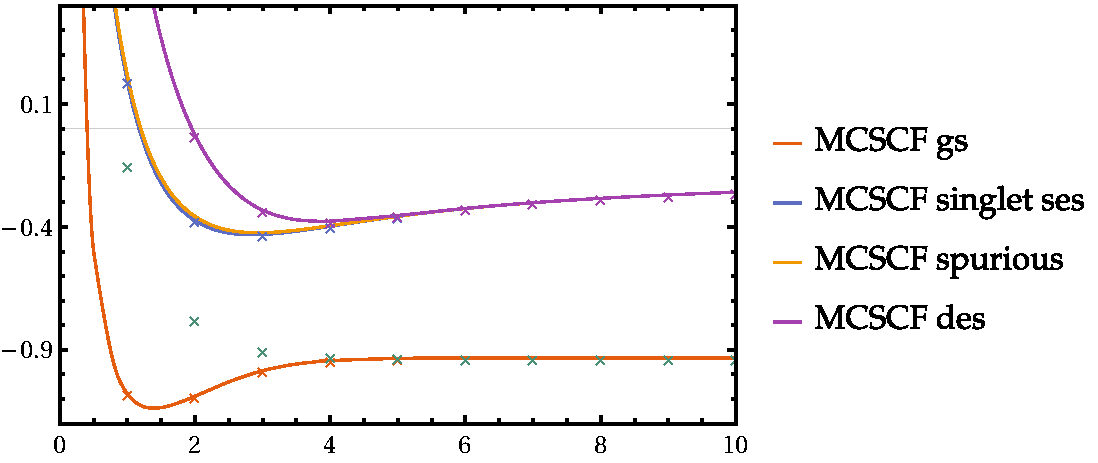
\includegraphics[width=0.67\linewidth]{Figures/H2_ooCID_PES}
  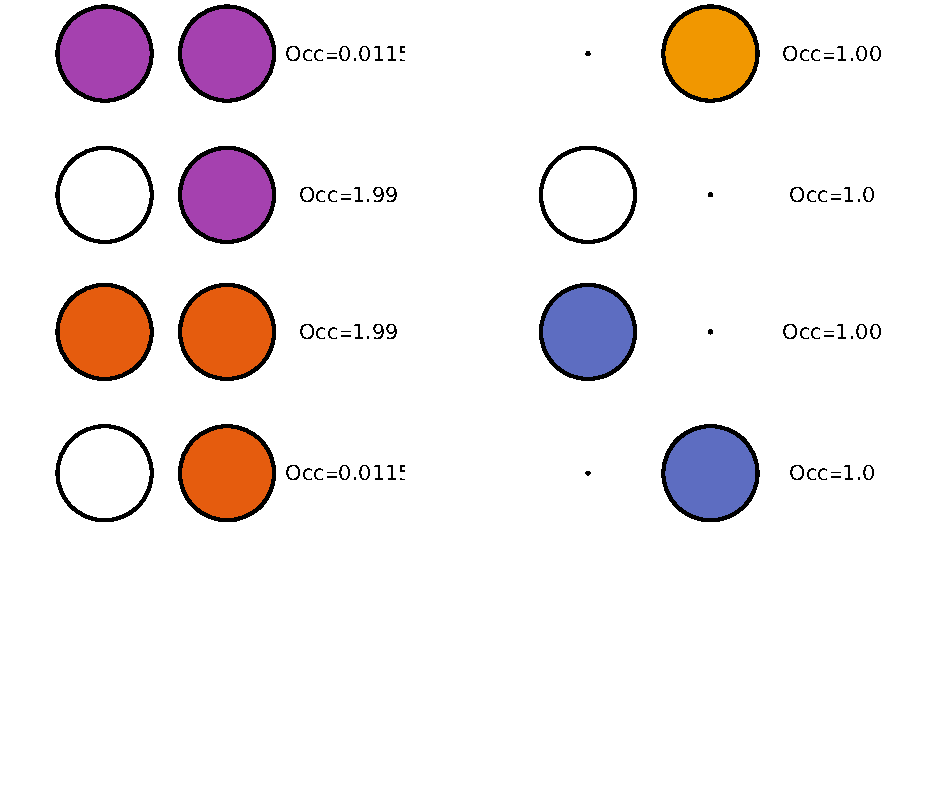
\includegraphics[width=0.32\linewidth]{Figures/H2_ooCID_MO}
  \caption{
    Energies (in hartree) of various oo-CID solutions as functions of the bond length $R$ (in bohr) for the \ce{H2} molecule in the STO-3G basis set.
    \label{fig:H2ooCID}}
\end{figure}
%%% %%% %%% %%%

Next we turn our attention to the two other ansatz. The oo-SACIS gives 5 solutions, three of which correspond to genuine RHF solutions. The two others are the ground state (with symmetry broken natural  orbitals) and the exact singlet singly excited state with symmetry pure orbital.
By adding some flexibility to the wave function, we see that the oo-CIS ansatz yields also the exact triplet. In addition, we also see some UHF some solution even if we are still in a RHF formalism.
%%% FIG 2 %%%
\begin{figure}
  \centering
  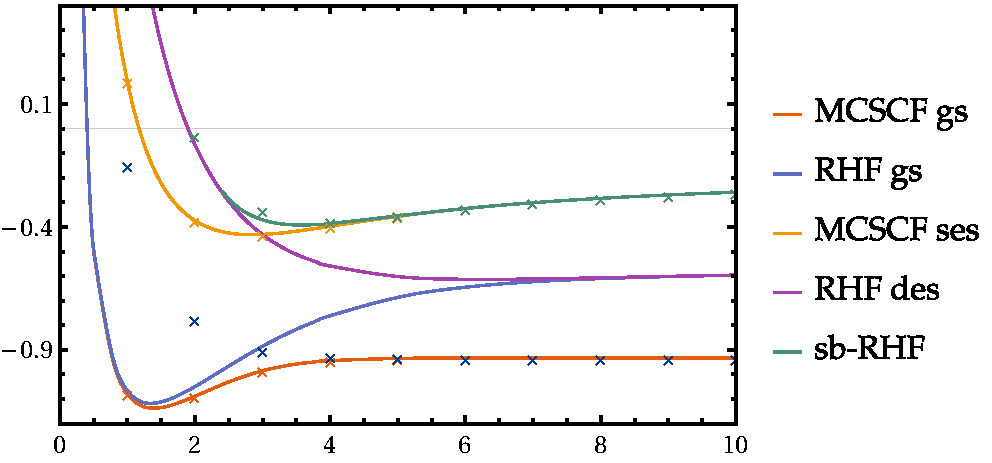
\includegraphics[width=0.75\linewidth]{Figures/H2_ooSACIS_PES}
  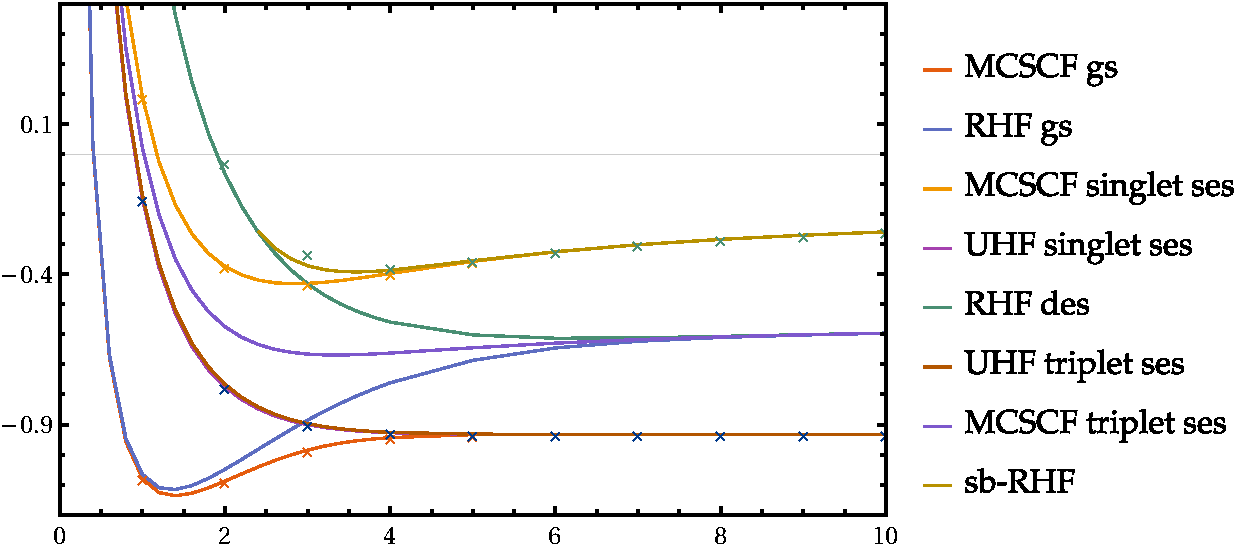
\includegraphics[width=0.75\linewidth]{Figures/H2_ooCIS_PES}
  \caption{
    Energies (in hartree) of various oo-SACIS and oo-CIS solutions as functions of the bond length $R$ (in bohr) for the \ce{H2} molecule in the STO-3G basis set.
    \label{fig:H2ooCIS}}
\end{figure}
%%% %%% %%% %%%

\textbf{Investigation of the spurious solution}

We want to know if the additional solution is a true unphysical solution due to approximate level of theory or if it is a mathematical spurious solution.
One cause of the latter type of solutions is that the tangent space can be ill-defined at certain point of the landscape. These points are therefore parametrization dependent.

We will start with the oo-CID wave function. In this very simple case, we can compute the two tangent vectors exactly.
\begin{align}
  \label{eq:H2_TangentVectors}
  \ket{\eta_1} &= e^{\hK} \left(\ketbra{\sigma_u\bar{\sigma}_u}{\sigma_g\bar{\sigma}_g} -\ketbra{\sigma_g\bar{\sigma}_g}{\sigma_u\bar{\sigma}_u}\right)\ket{\sigma_g\bar{\sigma}_g} = e^{\hK} \ket{\sigma_u\bar{\sigma}_u} \\
  \ket{\eta_2} &= \left(\cre{u}\ani{g} - \cre{g}\ani{u}\right)e^{\hS}\ket{\sigma_g\bar{\sigma}_g} = \left(\cre{u}\ani{g} - \cre{g}\ani{u}\right)\left(\cos(\phi)\ket{\sigma_g\bar{\sigma}_g} + \sin(\phi)\ket{\sigma_u\bar{\sigma}_u}\right) \\
               &= \cos(\phi)\left(\ket{\sigma_u\bar{\sigma}_g}-\ket{\bar{\sigma}_u\sigma_g}\right) - \sin(\phi)\left(\ket{\sigma_g\bar{\sigma}_u}-\ket{\bar{\sigma}_g\sigma_u}\right) \\
  &= \left(\sin(\phi)-\cos(\phi)\right)\ket{\bar{\sigma}_g\sigma_u} + \left(\cos(\phi)-\sin(\phi)\right)\ket{\sigma_g\bar{\sigma}_u} = 0~\text{if}~\phi = \frac{\pi}{4} + 2n\pi,~\forall n\in \mathbb{Z}
\end{align}
We can then compute the metric matrix elements
\begin{align}
  \braket{\eta_1}{\eta_1} &= 1 \\
  \braket{\eta_2}{\eta_2} &= 2(\sin(\phi)-\cos(\phi))^2 \\
  \braket{\eta_1}{\eta_2} &= \bra{\sigma_u\bar{\sigma}_u}e^{-\hK}\mleft[\left(\sin(\phi)-\cos(\phi)\right)\ket{\bar{\sigma}_g\sigma_u} + \left(\cos(\phi)-\sin(\phi)\right)\ket{\sigma_g\bar{\sigma}_u}\mright]
\end{align}

%%%%%%%%%%%%%%%%%%%%%%%%%%%%%%%%%%%%%%%%%%%%%%%%%%
\subsection{Linear \ce{HHe+}}
%%%%%%%%%%%%%%%%%%%%%%%%%%%%%%%%%%%%%%%%%%%%%%%%%%

The case of \ce{HHe+} is analog to \ce{H2}. Yet, we see a difference at large $R$ which is that the spurious solution does not coalesce with the doubly excited state.
The singly excited state and the spurious solution are more localized than the natural orbitals of the ground and doubly excited states (we cannot say symmetry broken because the system is not symmetric\dots). 

\begin{figure}
  \centering
  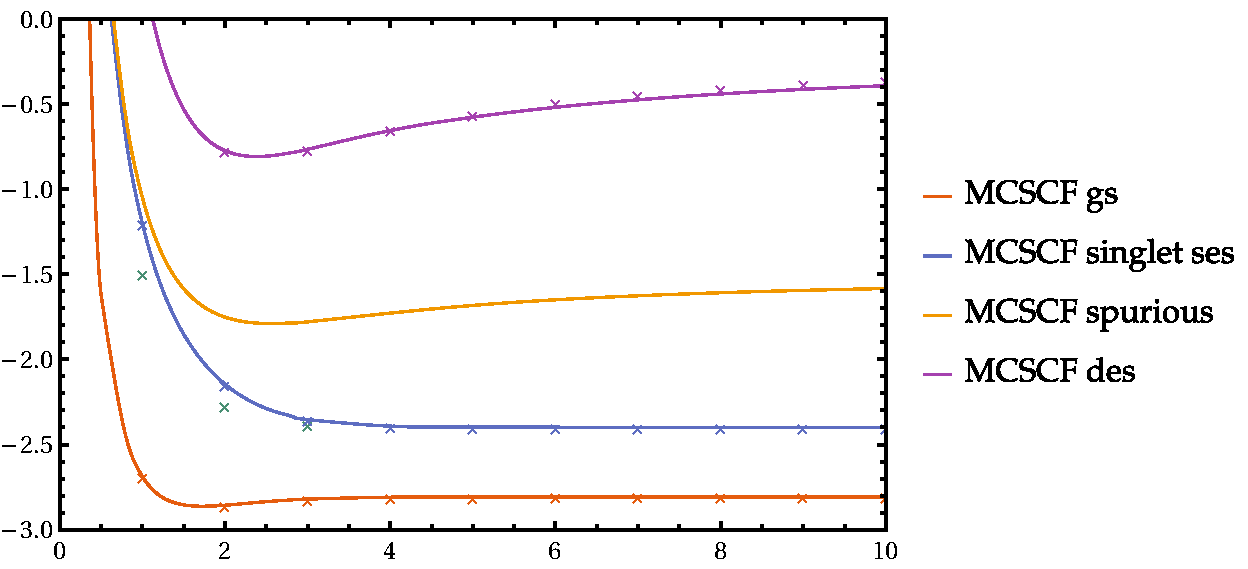
\includegraphics[width=0.75\linewidth]{Figures/HHe_ooCID_PES}
  \caption{
    Energies (in hartree) of various oo-CID solutions as functions of the bond length $R$ (in bohr) for the \ce{HHe+} molecule in the STO-3G basis set.
    \label{fig:HHeooCID}}
\end{figure}

%%%%%%%%%%%%%%%%%%%%%%%%%%%%%%%%%%%%%%%%%%%%%%%%%%
\subsection{Linear \ce{H3}}
%%%%%%%%%%%%%%%%%%%%%%%%%%%%%%%%%%%%%%%%%%%%%%%%%%

We now turn to a slightly larger molecule, namely the linear \ce{H3-} molecule in the STO-3G basis set.
We start by focusing on this system at R=1 bohr. This system has 9 exact FCI solutions as you can see below. At R=1 there are three HF solutions.
We also add the CASSCF(2,2) solutions closest to the FCI solutions in terms of energy. However, in this case there are additional solutions as we will see in more details below.

\begin{table}[h!]
  \begin{center}
    \caption{FCI energies and Hartree-Fockk}
    \label{tab:table1}
    \begin{tabular}{l|c|c|c|c|c|c|c|c|c}
      \textbf{FCI} & -0.848420 & 0.551175 & 0.779721 & 1.21422 & 1.43229 & 2.38312 & 2.77926 & 3.12430 & 3.62074 \\
      \textbf{Spin mult} & S & T & S & T & S & S & T & S & S \\
      \hline
      \textbf{HF} & -0.840048 &  &  &  &  & 2.36827 &  &  & 3.59501 \\
      \hline
      \textbf{CASSCF} & -0.845204 &  & 0.779721 &  & 1.46457 & 2.37341 &  & 3.12430 & 3.61641 \\
    \end{tabular}
  \end{center}
\end{table}

We will now focus on the CASSCF solutions, especially on the unphysical solutions. We will compare the CASSCF results with a MCSCF wave function. Both wave function are given below. One should be careful that the exponential operator in the CAS case does not have the active active rotation.
\begin{align}
  \ket{\Psi_\text{CAS}} &= e^{\hK_\text{CAS}}\left(\cos(\phi_1)\cos(\phi_2)\ket{1\bar{1}2\bar{2}} + \frac{\sin(\phi_1)\cos(\phi_2)}{\sqrt{2}}(\ket{1\bar{1}2\bar{3}}-\ket{1\bar{1}3\bar{2}}) + \sin(\phi_2)\ket{1\bar{1}3\bar{3}}\right) \\
  \ket{\Psi_\text{MC}} &= e^{\hK_{\text{MC}}}\left(\cos(\phi_1)\ket{1\bar{1}2\bar{2}} + \sin(\phi_1)\ket{1\bar{1}3\bar{3}}\right)
\end{align}
In addition, we will also compare two parametrizations of the orbital rotation operator namely the exponential parametrization and the Givens parametrization.

\textbf{Ground state}

The ground state energy is the same for all 4 methods considered here. In addition, the natural orbitals are also common to all methods (left below).
In all methods, we also found a stationary point which lie closely above the ground state. The corresponding energy as well as the orbitals are given below.

\begin{minipage}{0.3\textwidth}
  \centering
  \captionof{table}{FCI, CASSCF and MCSCF energies}
  \begin{tabular}{r|c c}
    \textbf{FCI} & -0.848420 & \\
    \hline
    \textbf{CASSCF} & -0.845204 & -0.843608 \\
    \hline
    \textbf{MCSCF} & -0.845204 & -0.843608
  \end{tabular}
\end{minipage}
\hfill
\begin{minipage}{0.6\textwidth}
  \centering
  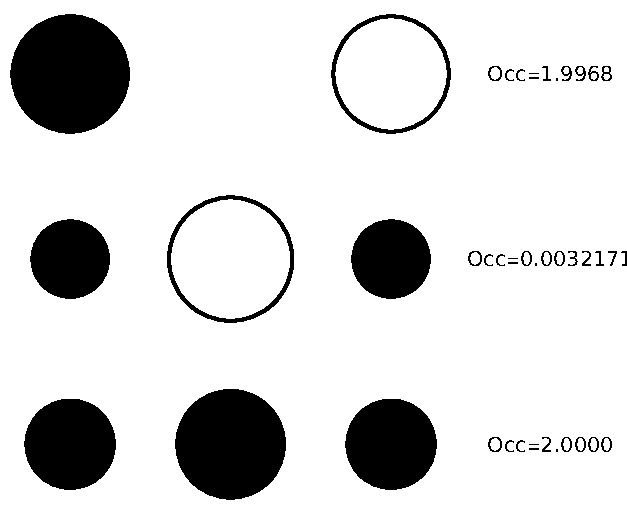
\includegraphics[width=0.49\linewidth]{Figures/H3_GS1_NO}
  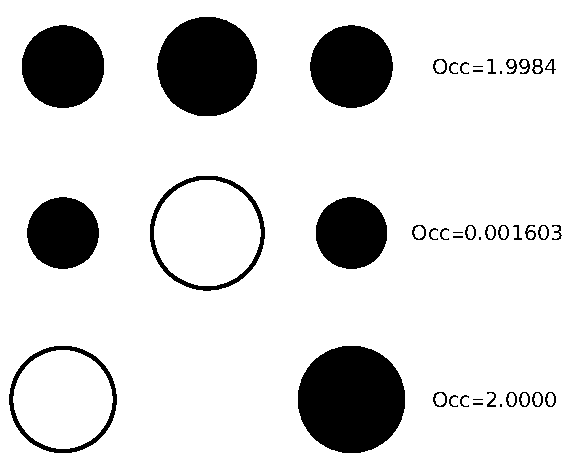
\includegraphics[width=0.49\linewidth]{Figures/H3_GS2_NO}
  \captionof{figure}{Natural orbitals of the ground state solutions.}
  \label{fig:H3_GS_NO}
\end{minipage}

\textbf{First excited state}

The first singly excited state can be obtained exactly by both wave functions using both parametrizations. Yet, we see a difference in the natural orbitals. Below, we see that the CASSCF natural orbitals (left) are symmetry-pure, whereas the MCSCF wave function has two symmetry-broken natural orbitals. Yet the overall MCSCF wave function is symmetry pure. In addition, MCSCF exhibit an unphysical solution with the same symmetry-broken orbitals but one of them is sign flip.
\begin{table}
  \begin{center}
    \caption{FCI, CASSCF and MCSCF energies}
    \label{tab:table1}
    \begin{tabular}{r|c c}
      \textbf{FCI} & 0.779721 & \\
      \hline
      \textbf{CASSCF} & 0.779721 & \\
      \hline
      \textbf{MCSCF} & 0.779721 & 0.886230
    \end{tabular}
  \end{center}
\end{table}
\begin{figure}
  \centering
  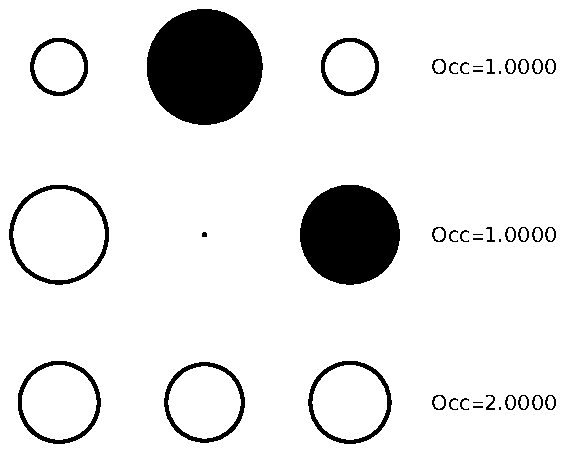
\includegraphics[width=0.28\linewidth]{Figures/H3_ES1_CAS_NO}
  \hspace{0.65cm}
  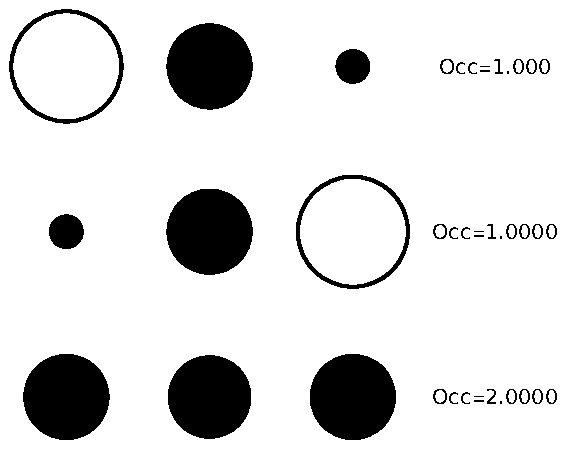
\includegraphics[width=0.28\linewidth]{Figures/H3_ES1_MC1_NO}
  \hspace{0.65cm}
  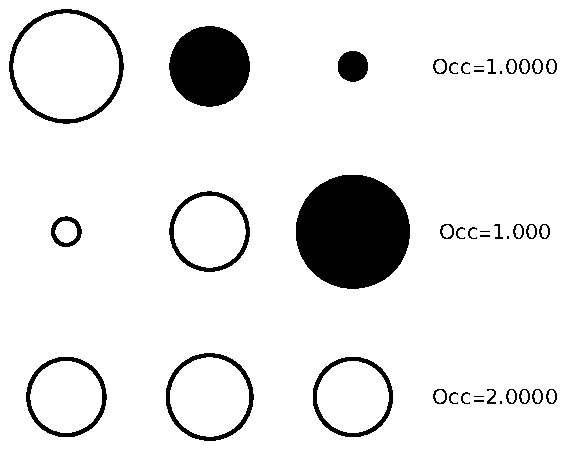
\includegraphics[width=0.28\linewidth]{Figures/H3_ES1_MC2_NO}
  \caption{
    Natural orbitals of the first excited state solutions.
    \label{fig:H3_ES1_NO}}
\end{figure}

\textbf{Second excited state}

\begin{minipage}{0.3\textwidth}
  \centering
  \captionof{table}{FCI, CASSCF and MCSCF energies}
  \begin{tabular}{r|c c}
      \textbf{FCI} & 1.43229 & \\
      \hline
      \textbf{CASSCF} & 1.46457 & \\
      \hline
      \textbf{MCSCF} & 1.46457 & 1.50262
    \end{tabular}
\end{minipage}
\hfill
\begin{minipage}{0.6\textwidth}
  \centering
  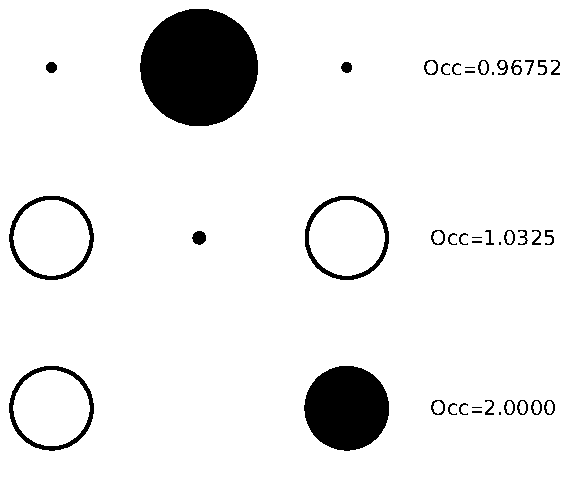
\includegraphics[width=0.49\linewidth]{Figures/H3_ES2_CAS_NO}
  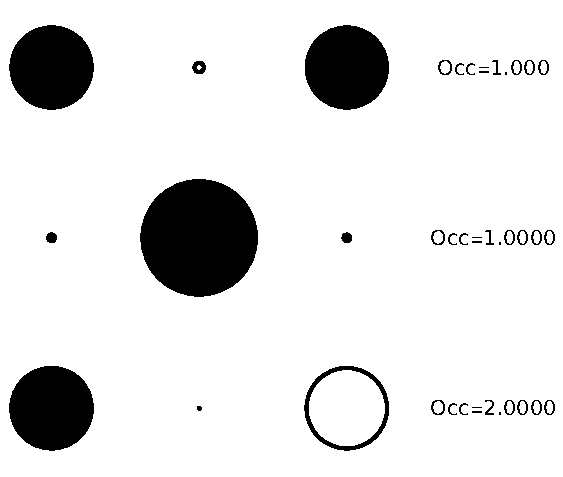
\includegraphics[width=0.49\linewidth]{Figures/H3_ES2_MC_NO}
  \captionof{figure}{Natural orbitals of the second excited state solutions.}
  \label{fig:H3_ES2_NO}
\end{minipage}

\textbf{Third excited state}

\begin{minipage}{0.3\textwidth}
  \centering
  \captionof{table}{FCI, CASSCF and MCSCF energies}
  \begin{tabular}{r|c c}
    \textbf{FCI} &  & 2.38312 \\
    \hline
    \textbf{CASSCF} & 2.36122 & 2.36851 \\
    \hline
    \textbf{MCSCF} & 2.36122 & 2.36851 \\
    \hline
    \textbf{Givens} & 2.34815 & 
  \end{tabular}
\end{minipage}
\hfill
\begin{minipage}{0.6\textwidth}
  \centering
  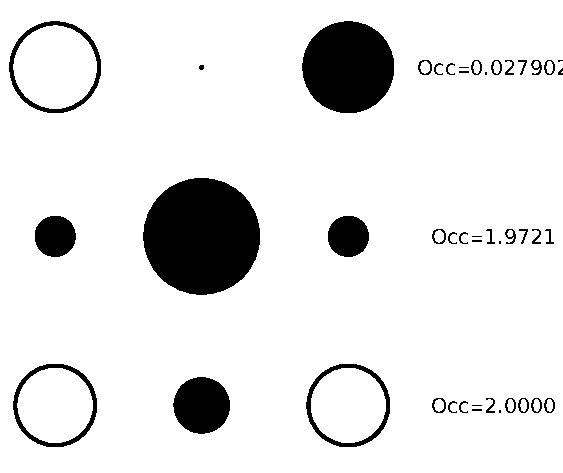
\includegraphics[width=0.49\linewidth]{Figures/H3_ES3_1_NO}
  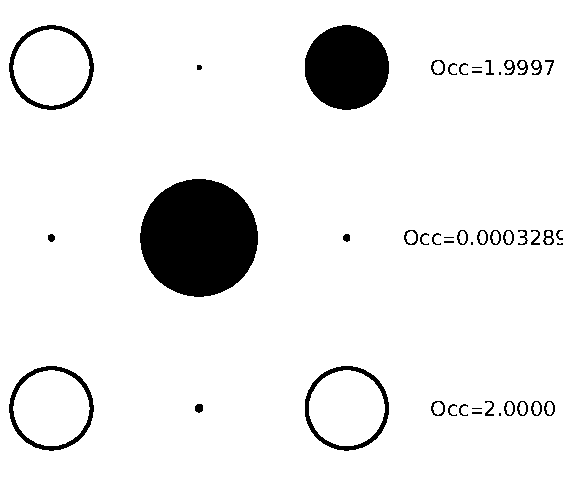
\includegraphics[width=0.49\linewidth]{Figures/H3_ES3_2_NO}
  \captionof{figure}{Natural orbitals of the third excited state solutions.}
  \label{fig:H3_ES3_NO}
\end{minipage}

\textbf{Forth excited state}

The situation for the forth excited state is the same as for the first one. Yet we see an additional solution for wave funtion with the Givens parametrisation. This solution is also symmetry broken, see the right panel of fig.\ref{fig:H3_ES4_NO}.
\begin{table}
  \begin{center}
    \caption{FCI, CASSCF and MCSCF energies}
    \label{tab:table1}
    \begin{tabular}{r|c c}
      \textbf{FCI} & 3.12430 & \\
      \hline
      \textbf{CASSCF} & 3.12430 & \\
      \hline
      \textbf{MCSCF} & 3.12430 & 3.15160 \\
      \hline
      \textbf{Givens} & 3.09589 &
    \end{tabular}
  \end{center}
\end{table}
\begin{figure}
  \centering
  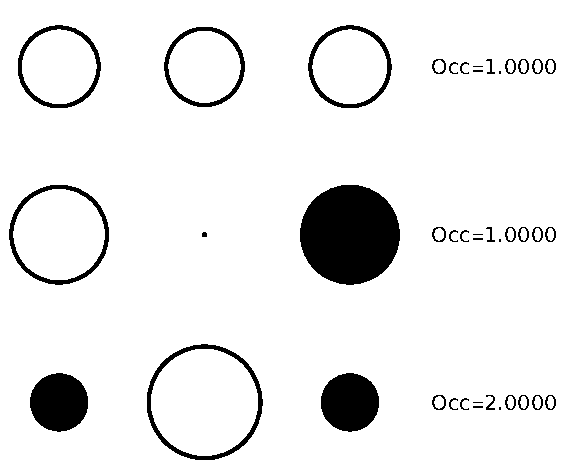
\includegraphics[width=0.28\linewidth]{Figures/H3_ES4_CAS_NO}
  \hspace{0.65cm}
  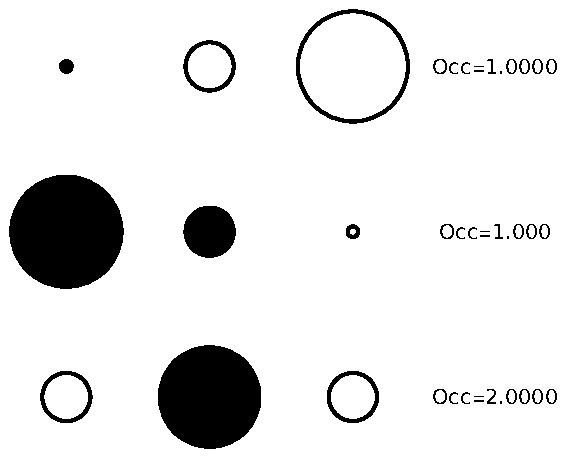
\includegraphics[width=0.28\linewidth]{Figures/H3_ES4_MC1_NO}
  \hspace{0.65cm}
  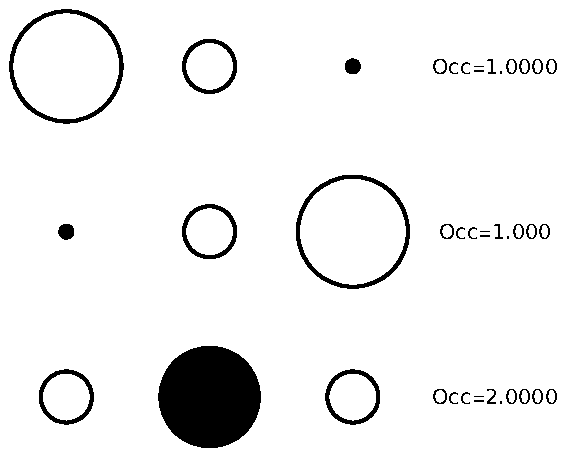
\includegraphics[width=0.28\linewidth]{Figures/H3_ES4_MC2_NO}
  \caption{
    Natural orbitals of the forth excited state solutions.
    \label{fig:H3_ES4_NO}}
\end{figure}

\textbf{Fifth excited state}

The fifth excited state lies in a really flat region of space. There is maybe other non-physical solutions around this one but consistent convergence toward them is really hard with the present algorithm.
\begin{minipage}{0.3\textwidth}
  \centering
  \captionof{table}{FCI, CASSCF and MCSCF energies}
  \begin{tabular}{r|c}
    \textbf{FCI} & 3.62074 \\
    \textbf{CASSCF} & 3.61641 \\
    \textbf{MCSCF} & 3.61641
  \end{tabular}
\end{minipage}
\hfill
\begin{minipage}{0.6\textwidth}
  \centering
  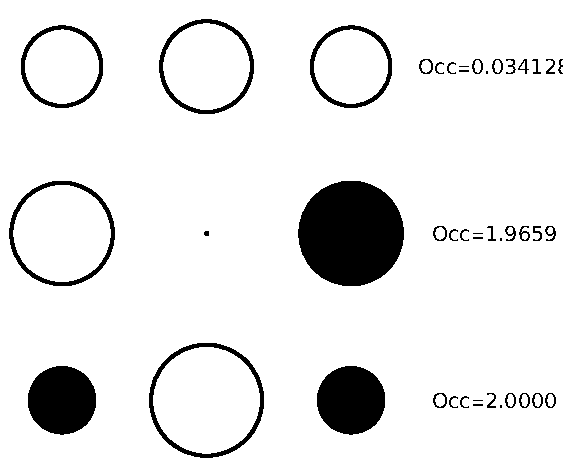
\includegraphics[width=0.49\linewidth]{Figures/H3_ES5_CAS_NO}
  \captionof{figure}{Natural orbitals of the fifth excited state solutions.}
  \label{fig:H3_ES5_NO}
\end{minipage}

\textbf{Givens stationary points}

\begin{figure}
  \centering
  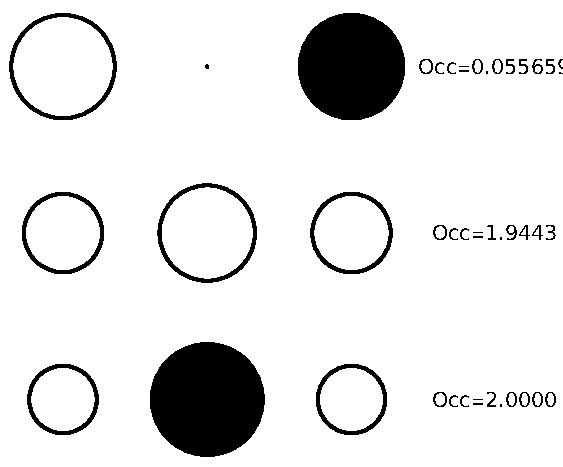
\includegraphics[width=0.28\linewidth]{Figures/H3_Givens1_NO}
  \hspace{0.65cm}
  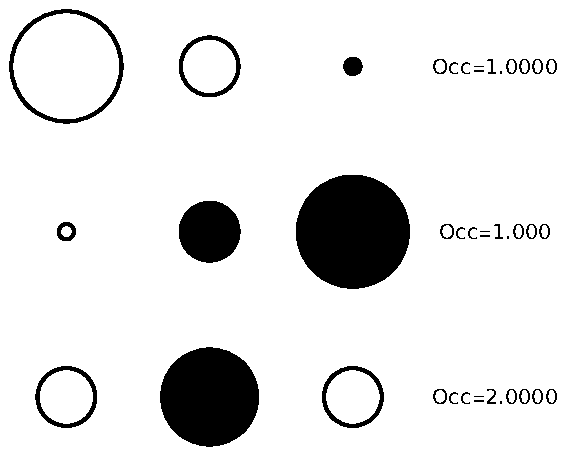
\includegraphics[width=0.28\linewidth]{Figures/H3_Givens2_NO}
  \caption{
    Natural orbitals of spurious solutions found with the Givens parametrization.
    \label{fig:H2ooCIS}}
\end{figure}

%=================================================================%
\section{MOM-MCSCF}
\label{sec:MOM-MCSCF}
%=================================================================%

%%%%%%%%%%%%%%%%%%%%%%%%%%%%%%%%%%%%%%%%%%%%%%%%%%
\subsection{Subsec}
%%%%%%%%%%%%%%%%%%%%%%%%%%%%%%%%%%%%%%%%%%%%%%%%%%

%=================================================================%
\section{Perturbation theory on a periodic landscape}
\label{sec:PT}
%=================================================================%

%=================================================================%
\section{Miscellaneous}
\label{sec:misc}
%=================================================================%

\end{document}